\section{Descripició del/s motor/s}
Les característiques que ha de complir el motor son les següents:
\begin{itemize}
\item Empenta de creuer: $F=25000N$
\item Alçada de vol: $h=9500m$
\item Velocitat de creuer: $v=600km/h$
\end{itemize}
A més de tot això es tracta d'un disseny real, per la qual cosa s'han de tenir en compte els següents ratis i temperatura màxima d'entrada a la turbina:
\begin{itemize}
\item Rati de pressió al difusor: $\pi_d=0.96$
\item Rendiment al compressor: $\eta_c=0.88$
\item Rati de pressió a la cambra de combustió: $\pi_b=0.94$
\item Eficiència de combustió: $\eta_b=0.99$
\item Rendiments de turbina: $\eta_{tH}=\eta_{tL}=0.87$
\item Rati de pressió a la tovera: $\pi_n=0.98$
\item Rendiment mecànic: $\eta_{mec}=0.99$
\item Temperatura d'entrada a la turbina: $T_{t4}=1780$
\end{itemize}
Sample Figure
\begin{figure}[H]
	\centering
	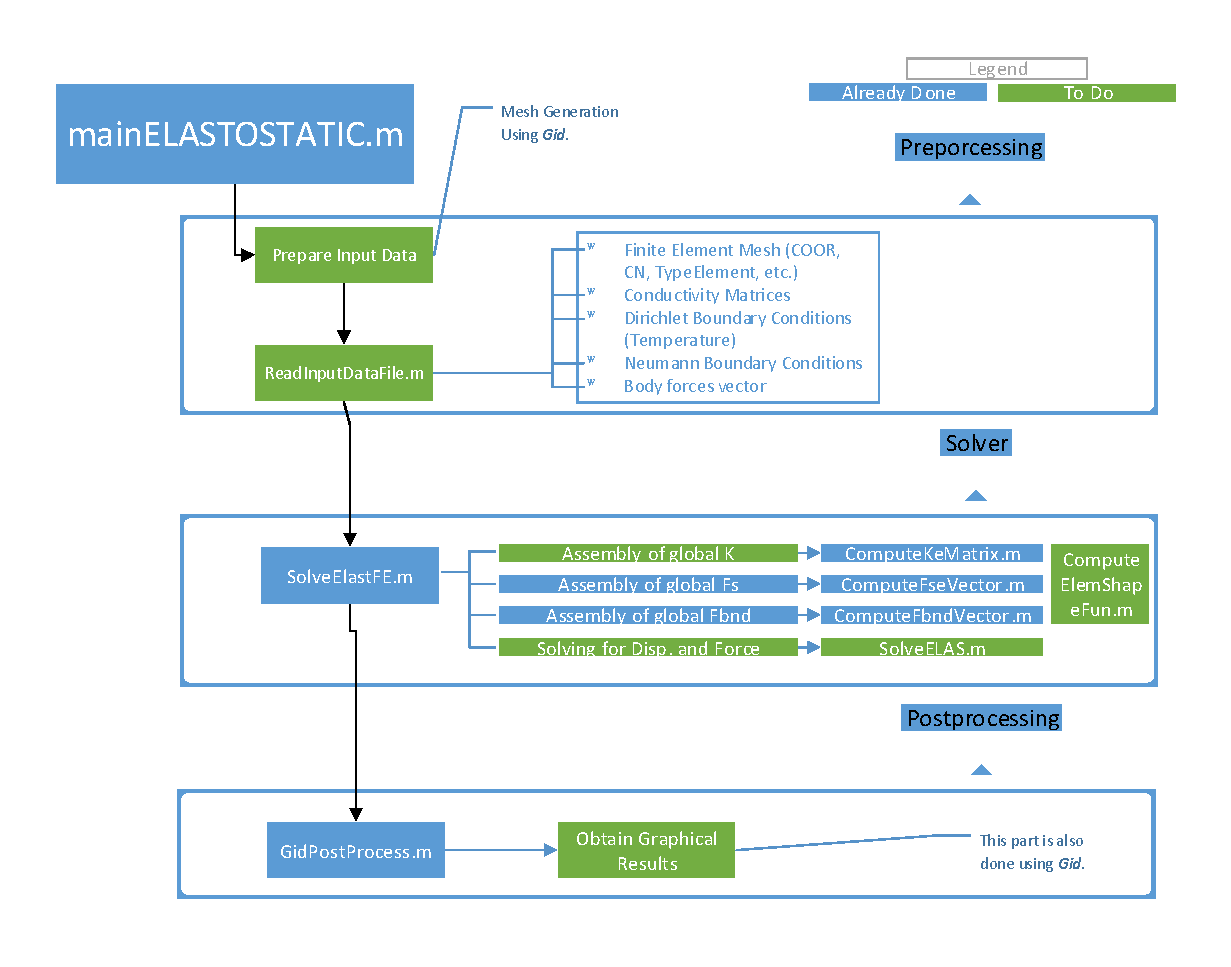
\includegraphics[scale=0.9]{./pics/sample}
	\caption{Sample Caption}
\end{figure}
Numbered equation:
\begin{equation}
	K^e = \sum_{g=1}^{m}w_g (J^eB^{e^T}C B^e)_{\xi=\xi_g}
\end{equation}
In line equation:
final Global stiffness matrix K dimensions will be $n_{sd}n_{pt}\times n_{sd}n_{pt}$.
Amb les dades disponibles de velocitat de creuer i altitud podem assimilar que el tipus d'aeronau per al qual va destinat es un avió de negocis lleuger, com pot ser el Cessna 510 Citation Mustang. 



Sample Listing:
\lstinputlisting[caption={ComputeK.m},label={ComputeK}]{./code/sample.m}
